\chapter{Høreapperatet}\label{ch:apperatet}
\section{Høreapperatet}
Hørerapperatet er som beskrevet i afsnit \ref{ch:Teori} bestående af båndpas-filtre. Der opdeler input-signalet i frekvensbånd, der bliver vægtet forskelligt før de bliver sat sammen til et output-signal.

Der er blevet lavet et Matlab program, hvor der først bliver foretaget en Diskret Fourrier Transformation på indgangssignalet for at finde ud af, hvilke frekvenser indgangsignalet indeholder.
Efterfølgende bliver inputsignalet kørt igennem det fremstillede Hørerapperats filter. Efter det er blevet kørt igennem filteret bliver output-signalet også Diskret Fourrier Transformeret, så der kan overskues, hvilke frekvenskarakteristika dette signal indeholder.
\section{Matlab kode for de forskellige funktioner}
\subsection{FIR-Båndpass funktion}
\begin{verbatim}
 function [ output_signal, filter1] = FIR_bandpass_function(input_signal,fc1,fc2 )
 
 len = length(input_signal);
 
 fs = 48000;
 
 N = 1000;
 
 df = fs/N;
 
 m1 = round(fc1/df); %bin nummer der passer bedst
 m2 = round(fc2/df); %-||-
 
 filter1 = [zeros(1,m1) ones(1,abs(m1-m2)) zeros(1,N/2-m1-abs(m1-m2))];
 filter1 = [filter1 zeros(1,N/2-m1-abs(m1-m2)) ones(1,abs(m1-m2)) zeros(1,m1)];
 
 filter_time = fftshift(real(ifft(filter1)));
 
 x1 = filter(filter_time,1,input_signal);
 
 hann = hanning(len)';
 
 output_signal = x1.*hann;
 
 end
\end{verbatim}

 
\subsection{IIR-bandpass filter}
Der blev designet et lavpas-filter i matlab ved brug af Matlabs Filter Design and Analysis Tool. Indstillingerne, der blev sat og det vedhæftede fase og amplitude response kan ses på billede 

Filteret blev desginet med ønske i at skabe et IIR butterworth filter med to knækfrekvens på 300Hz til 400 Hz og er andenorsdens. 
Da filteret var designet blev koefficenterne exporteret til et matlab-fil, der blev benyttet i funktionen IIR-lowpass filter.

\begin{figure}[H]
	\centering
	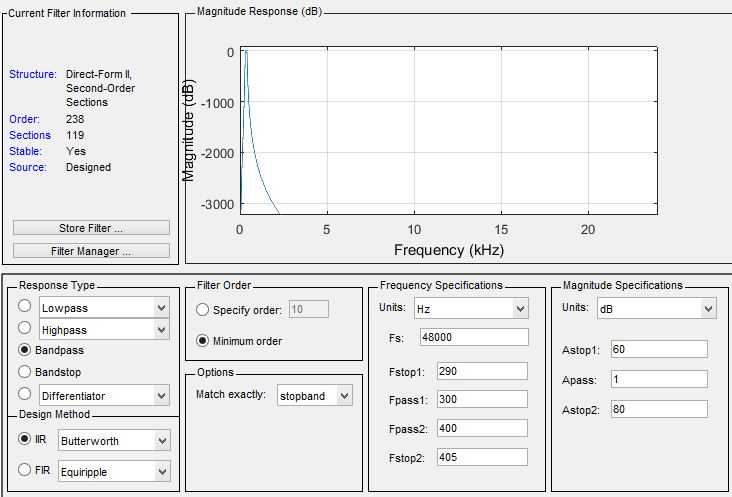
\includegraphics[width=150mm]{figures/IIRlavpas.jpg}
	\caption{Design af IIR lavpas filter i FDA tools i matlab}
	\label{fig:FDAtools}
\end{figure}

Filteret blev desginet med ønske i at skabe et IIR butterworth filter med en knækfrekvens på 10Hz og med en orden på 10. 
Da filteret var designet blev filteret exporteret til en matlab-funktion gennem matlabs indbyggede code generator der blev benyttet i funktionen IIR-lowpass filter.

Koden for IIR lavpas filter funktionen kan ses nedenuner:
\begin{verbatim}
	function Hd = IIR_lavpas
	%IIR_LAVPAS Returns a discrete-time filter object.
	
	% MATLAB Code
	% Generated by MATLAB(R) 9.0 and the Signal Processing Toolbox 7.2.
	% Generated on: 10-May-2016 12:59:58
	
	% Butterworth Bandpass filter designed using FDESIGN.BANDPASS.
	
	% All frequency values are in Hz.
	Fs = 48000;  % Sampling Frequency
	
	Fstop1 = 290;         % First Stopband Frequency
	Fpass1 = 300;         % First Passband Frequency
	Fpass2 = 400;         % Second Passband Frequency
	Fstop2 = 405;         % Second Stopband Frequency
	Astop1 = 60;          % First Stopband Attenuation (dB)
	Apass  = 1;           % Passband Ripple (dB)
	Astop2 = 80;          % Second Stopband Attenuation (dB)
	match  = 'stopband';  % Band to match exactly
	
	% Construct an FDESIGN object and call its BUTTER method.
	h  = fdesign.bandpass(Fstop1, Fpass1, Fpass2, Fstop2, Astop1, Apass, ...
	Astop2, Fs);
	Hd = design(h, 'butter', 'MatchExactly', match);
	
	% [EOF]
	
	
	
	ans =
	
	FilterStructure: 'Direct-Form II, Second-Order Sections'
	Arithmetic: 'double'                               
	sosMatrix: [119x6 double]                         
	ScaleValues: [120x1 double]                         
	OptimizeScaleValues: true                                   
	PersistentMemory: false
	
\end{verbatim}

\subsection{Weight funktion}

Høreapperatet blev kørt med forskellige signaler, hvor der blev eksperimenteret med forskellige vægtning af de enkelte Båndpas-filtre samt frekvensbåndet, de enkelte filtre dækkede. Efter at havde eksperimenteret med de forskellige frekvensbånd blev det bestemt, at de enkelte frekvensbånd skulle dække følgende frekvensområder, der alle ligger i det hørbare frekvensområde:
\begin{itemize}
	\item Bånd 1 - 300-400 Hz
	\item Bånd 2 - 400-600 Hz
	\item Bånd 3 - 600-1000 Hz
	\item Bånd 4 - 1000-2000Hz
	\item Bånd 5 - 2000-3400 Hz
\end{itemize}

Koden til weight-funktionen:
\begin{verbatim}

%Give weights in dB
function [ output_signal ] = WEIGHT_func(input_signal,weight,weight2,weight3,weight4,weight5)
% Opdeler signalet i 5 forskellige frekvensbånd, der ligger i båndet for
% menneskeligt tale

x = IIR_lavpas();
b1=x.sosMatrix(:,5);
a1=x.sosMatrix(:,6);
[LP] = filter(b1,a1,input_signal);

[BP1, ~] = FIR_bandpass_function(input_signal, 400, 600);
[BP2, ~] = FIR_bandpass_function(input_signal, 600, 1000);
 x1 = hoereapparat; %1000-2000Hz
 b2=x1.sosMatrix(:,5);
 a2=x1.sosMatrix(:,6);
 [BP3] = filter(b2,a2,input_signal);

 x2 = IIR_highpas(); %2000-3400Hz
 b3=x2.sosMatrix(:,5);
 a3=x2.sosMatrix(:,6);
 [HP] = filter(b3,a3,input_signal);

% Vægt de 5 forskellige frekvens bånd, så de tilpasser sig til personens
% individuelle behov:
LP = LP * weight;
BP1 = BP1 * weight2;
BP2 = BP2 * weight3;
BP3 = BP3 * weight4;
HP = HP * weight5;

clc;
figure(1)
subplot(5,1,1)
plot(LP);
subplot(5,1,2)
plot(BP1);
subplot(5,1,3)
plot(BP2);
subplot(5,1,4)
plot(BP3);
subplot(5,1,5)
plot(HP);

output_signal = LP + BP1 + BP2+ BP3+ HP;

output_signal = FIR_bandpass_function(output_signal,300,3400);

%[output_signal] = filter(b4,a4,input_signal);
\end{verbatim}



\subsection{Horeapparat}
\begin{verbatim}
%Høreapparat

[x, Fs]=audioread('Reporters.mp3');
N = 1000000;


%setup frekvensakse
fd = Fs/N;
x_akse = [0:fd:Fs-fd];

x = x(1:N);

x=rot90(x);

%Foretag FFT på signalet
X = fft(x);

y = WEIGHT_func(x,10,10,10,10,10);

%Foretag FFT på det vægtede signal
Y = fft(y);

%Plot de to signaler, så man kan se forskellen i frekvenserne.
% clc;
% figure(1)
% subplot(2,1,1)
% semilogx(x_akse(1:0.5*end),20*log10(abs((2/N)*X(1:0.5*end))));
% xlabel('Frekvens')
% ylabel('dB')
% subplot(2,1,2)
% semilogx(x_akse(1:0.5*end),20*log10(abs((2/N)*Y(1:0.5*end))));
% xlabel('Frekvens')
% ylabel('dB')

soundsc(x,Fs);
pause(10);
soundsc(y,Fs);
\end{verbatim}


I koden ses det at der sker en vægtning i forskellige frekvensbånd, og denne vægtning kan bruges til at møde den individulles behov, men kan også ændre på hvilke frekvensområder de enkelte bånd dækker over. Dette betyder at folk med forskellige hørerproblemer, kan få tilpasset et hørerapperat til netop deres behov.


\section{Resultat}
I dette afsnit fremstilles resultaterne af at køre Hørerapperatet på en række forskellige signaler. Signalet, der er blevet valgt at arbejde på er et lydklip af en nyhedsvært i stormvejr. I dette lydklip ønskes det at forstærke talen fra nyhedsværten og dæmpe baggrundsstøjen fra stormvejret.


De følgende billeder viser hvordan originalsignalet er blevet manipuleret, så frekvenserne i området 300-3400Hz er blevet forstærket mens de resterende frekvenser er blevet mindsket eller cuttet.   


\begin{figure}[H]
	\centering
	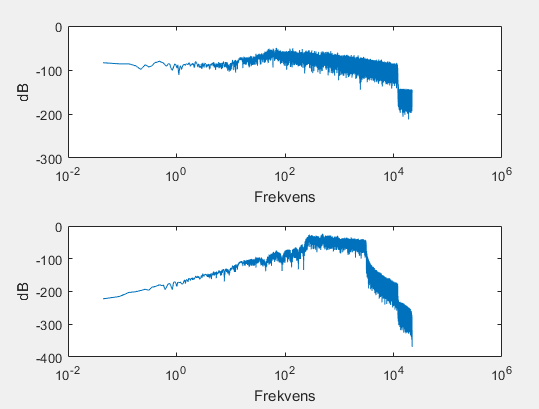
\includegraphics[width=150mm]{figures/hoereapparat_resultat.PNG}}
	\caption{frekvenser i hhv. det filtrerede og originale signal}
	\label{fig:Samlet frekvensplot}
\end{figure}


På fig \ref{fig:Samlet frekvensplot} ses at der i det filtrerede signal er frekvenserne indenfor bandpassende er forstærket, men frekvenser udenfor er væsentligt dæmpet.


\begin{figure}[H]
	\centering
	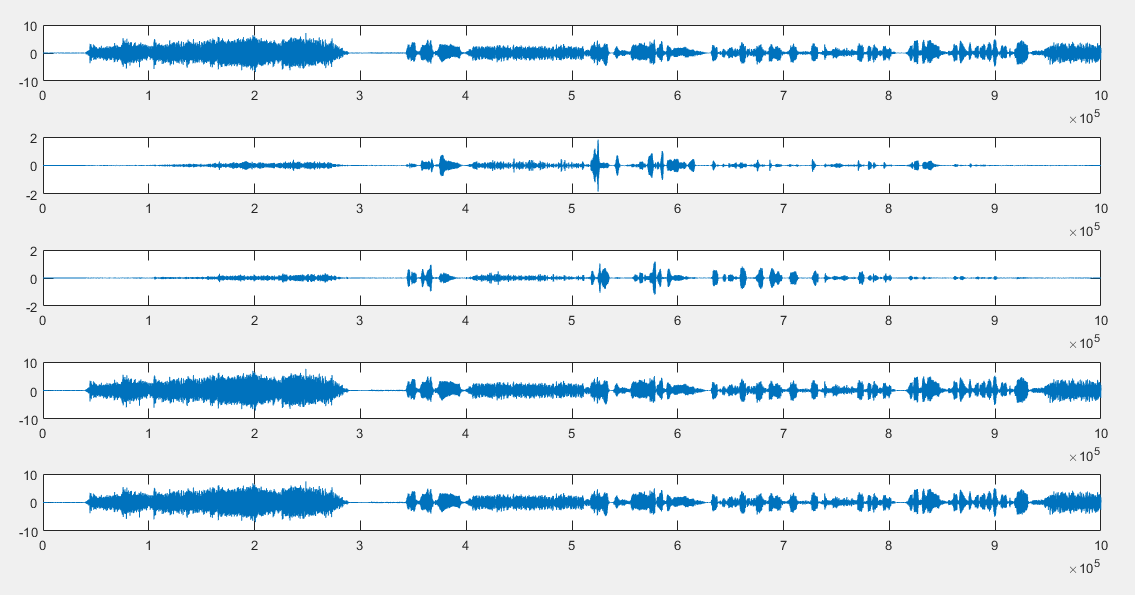
\includegraphics[width=150mm]{figures/indhold_i_band.PNG}}
	\caption{Indhold i de forskellige frekvensbånd}
	\label{fig:indholdiband}
\end{figure}


På fig \ref{fig:indholdiband} ses de fem bånd der bliver filtreret i, og det er dermed disse der kunne justeres. Evt. kunne sectionen udvides til flere bånd, men det er valgt ikke at blive gjort. 

